\subsection{Estabilidad de GeM}
\label{subsec:exp7}
\begin{LaTeXdescription}
    \item[Objetivo] Observar el ranking de PageRank/GeM puede sufrir variaciones
        importantes de una fecha a la otra, el recibir un set nuevo de
        informaci\'on.\\

    \item[Hip\'otesis] GeM es m\'as inestable que la puntuaci\'on oficial del
        f\'utbol.\\

    \item[Proposici\'on] Nos interesa considerar casos extremos para evaluar la
        estabilidad del ranking que devuelve GeM. El sistema de puntaje actual
        del f\'utbol tiene la caracter\'istica de ser bastante ''estable'': en
        una \'unica fecha un equipo puede ganar a lo sumo 3 puntos, lo cual
        (salvo en los comienzos de un torneo o casos de empate m\'ultiple
        dif\'iciles de encontrar en la realidad) no lo hace avanzar m\'as de 4 o
        5 posiciones.

        \par Nos interesa analizar si esta propiedad se conserva en GeM. Para
        eso, imaginemos un torneo de f\'utbol desbalanceado, es decir, un torneo
        que al finalizar, el primer equipo tiene mucha diferencia con el
        \'ultimo \footnote{Consideramos esto desbalanceado. Si no es este el
        caso del lector, simplemente considerar una instancia que cumpla con esa
        condici\'on.}. Si en una \'ultima fecha ''inventada'', u agregada
        artificialmente, el \'ultimo le ganase al primero, el m\'etodo de
        puntuaci\'on est\'andar dif\'icilmente altere demasiado el ranking.
        Queremos observar si esto ocurre con GeM.\\

    \item[M\'etodo de Experimentaci\'on] Tomamos el Campeonato de Primera B
        Nacional 2013/14, en el cual Banfield (1º) termin\'o con 78 puntos
        mientras que Villa San Carlos (22º y \'ultimo) termin\'o con 24.
        Generamos una fecha artificial extra en la que Villa San Carlos le Gana
        a Banfield 5 a 0. El ranking oficial no cambiar\'ia, dado que con 27
        puntos Villa San Carlos seguir\'ia \'ultimo. De confirmarse nuestra
        hip\'otesis, esperar\'iamos ver un cambio en la posición que GeM le
        asigna a Villa San Carlos. En este caso, variando la cantidad de goles,
        estudiamos cu\'anto se alterar\'ia el resultado si la victoria fuese
        a\'un m\'as abultada.\\

    \item[Resultados, an\'alisis y discusi\'on]
\end{LaTeXdescription}

\begin{wrapfigure}{r}{0.5\textwidth}
    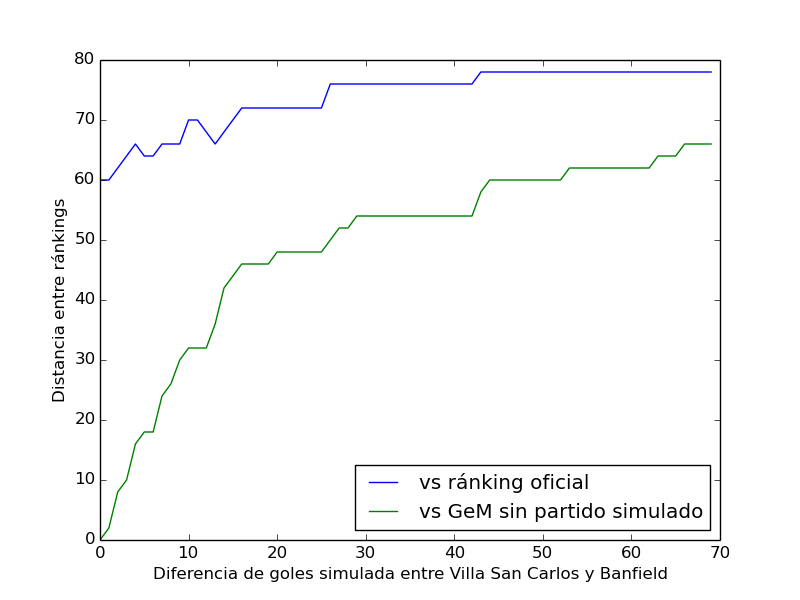
\includegraphics[width=0.5\textwidth]{exp7_diferencia_ranks_funcion_goles.png}
    \caption{Distancia Ranking GeM y Oficial vs Ranking GeM con partido Artificial}
    \label{fig:exp7_dist_ranks}
\end{wrapfigure}
\noindent

\par Ssaradara 
